\input{kls-cv-13}
%\ttfamily
\pagestyle{empty}

\begin{minipage}{.9\textwidth}
\section*{| Curriculum Vitae}
\vspace{3mm}
%\subsection*{| Personal Information}
\hspace{-4.5mm}
\begin{tabular}{ll}
	\begin{tabular}{ll}
		{\cmb \textbf{Name:}} & \textbf{Kim Timothy Engh}\\
		{\cmb \textbf{E-mail:}} & kimtengh@gmail.com\\
		{\cmb \textbf{Cell Phone:}} & {\cg(0047)} 40070995
	\end{tabular}
	&
	\begin{tabular}{lp{6cm}}
		{\cmb \textbf{Address:}} & Arendalsveien 19D,\newline 4878 GRIMSTAD,\newline Norway
	\end{tabular}
\end{tabular}
\end{minipage}
\begin{minipage}{.1\textwidth}
\vspace{-10mm}
\begin{flushright}
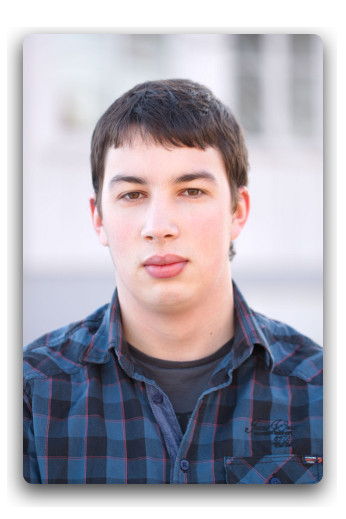
\includegraphics[scale=.75]{picture}
\end{flushright}
\end{minipage}

\tikzstyle{bar}=[rectangle, minimum size=.1mm, text width=1.02\textwidth, very thick, draw=white, top color=lightgray,bottom color=white!5!black!10]
\vspace{-2mm}

\begin{tikzpicture}
\node[bar]{};
\end{tikzpicture}

\subsection*{| Key features}
\hspace{-2.5mm}
\begin{tabular}{p{.3\textwidth}p{.7\textwidth}}
\rule[0ex]{0pt}{2.5ex}{\cmb\textbf{Work experience:}} & Over 5 years of experience as a service technician / field mechanic at Atlas Copco and in the Norwegian Army. I would for the most part troubleshoot and apply breakdown repairs on surface drilling rigs as well as other types of construction equipment. \\
\rule[2ex]{0pt}{2.5ex}{\cmb\textbf{Positions of trust:}} & I served as the union representative for the troop during my time in the Norwegian Army, and until recently I had a position at the board of Mekaunikum, the sorority for mechatronics at UiA.\\
\end{tabular}

\subsection*{| Education}
\hspace{-2.5mm}
\begin{tabular}{p{.3\textwidth}p{.7\textwidth}}
\rule[0ex]{0pt}{2.5ex}{\cmb\textbf{Bachelor, Mechatronics:}\newline{\cdg 2011-2014}} & I am currently studying mechatronics at the University in Agder, UiA. Expected graduation in 2014.\\
\rule[2ex]{0pt}{2.5ex}{\cmb\textbf{Atlas Copco:}\newline{\cdg 2006-2007}} & I worked as an apprentice at Atlas Copco finishing my education as a construction equipment mechanic. Test passed with highest grade.\\
\rule[2ex]{0pt}{2.5ex}{\cmb\textbf{High School:}\newline{\cdg 2003-2006}} & A 3 year mechanics education to be a construction equipment mechanic. Studied at Ås VGS and Solør VGS. 
\end{tabular}

\subsection*{| Work experience}
\hspace{-2.5mm}
\begin{tabular}{p{.3\textwidth}p{.7\textwidth}}
%\rule[0ex]{0pt}{2.5ex}{\cmb\textbf{Mekaunikum:}\newline{\cdg 2012-2013}} & Mekaunikum is the sorority for mechatronics students at UiA which I'm proud to be a part of. Our most important job is to connect students and employers. I was responsible for public relations and our web site.\\
\rule[2ex]{0pt}{2.5ex}{\cmb\textbf{Atlas Copco:}\newline{\cdg 2007-2011}} & Employed as a service technician working self-reliantly in the field. My tasks mostly consisted of troubleshooting, repairs, and training of customers. My field of expertise lies in surface drilling rigs.\\
\rule[2ex]{0pt}{2.5ex}{\cmb\textbf{Norwegian Army:}\newline{\cdg 2008}} & I served in the Engineer Battalion as a field mechanic, working in a team doing maintenance and breakdown repairs at camp and in the field. I also served as the union representative for my troop.
\end{tabular}

\subsection*{| Certificates / Training}
\hspace{-2.5mm}
\begin{tabular}{p{.3\textwidth}p{.7\textwidth}}
\rule[0ex]{0pt}{2.5ex}{\cdg }{\cmb\textbf{General certificates:}} & BE, C1E, C, M, T, T1, T2, T4, G4, G8, G20-F, M2, M4 \& hot work.\\
\rule[2ex]{0pt}{2.5ex}{\cmb\textbf{Atlas Copco Certified:}\newline{\cdg 2010}} & Certified Atlas Copco service technician. Training consists of courses about electrical systems, hydraulic control systems and specialized Atlas Copco technology.\\
\rule[2ex]{0pt}{2.5ex}{\cmb\textbf{Basic Engineer:}\newline{\cdg 2008}} & A course given by the Norwegian Army which consists of hands-on training with the armies construction equipment. The goal was to gain the required knowledge to operate and maintain a large number of machines.
\end{tabular}

\subsection*{| Other skills}
\hspace{-2.5mm}
\begin{tabular}{p{.3\textwidth}p{.7\textwidth}}
\rule[0ex]{0pt}{2.5ex}{\cdg }{\cmb\textbf{Languages:}} & My native language is Norwegian, but I also have good skills in English.\\
\rule[2ex]{0pt}{2.5ex}{\cdg}{\cmb\textbf{Computer skills:}} & I have very good computer skills and I know how to use several different operating systems, such as Linux, Windows and OS X. I also have experience with relevant applications such as $\LaTeX$, Solidworks, Scilab and Maxima.\\
\end{tabular}

\subsection*{| Personal interests}
	\hspace{-2.5mm}
	\begin{tabular}{p{.3\textwidth}p{.7\textwidth}}
		\rule[0ex]{0pt}{2.5ex}{\cdg }{\cmb\textbf{Photography:}} & My main interest lies in landscape photography. I also enjoy bringing my DSLR along while skiing slalom.\\
		\rule[2ex]{0pt}{2.5ex}{\cdg}{\cmb\textbf{Computing:}} & Currently i have a few projects based around the open hardware prototyping platform Arduino. This allows me to learn more about using electronic components as well as it's a good way to learn programming. I am writing code in C++ and python.
	\end{tabular}

\subsection*{| Attachments}
	\hspace{-2.5mm}
	\begin{tabular}{p{.3\textwidth}p{.7\textwidth}}
		\rule[0ex]{0pt}{2.5ex}{\cdg }{\cmb\textbf{Grades:}} & University in Agder, and certificate of completed apprenticeship.\\
		\rule[2ex]{0pt}{2.5ex}{\cdg}{\cmb\textbf{Letter of recommendation:}} & Atlas Copco, and the Norwegian Armed Forces.
	\end{tabular}
	
\subsection*{| Note}
Attachments and references can be delivered upon request in either digital or paper form. I also have a account at Linked-in. Thanks for taking the time to read my CV.

\end{document}
